\item Um homem de \SI{75}{\kilogram} salta para fora da plataforma circular com uma velocidade $v_{m/P}=\SI{1.5}{\meter/\second}$ em relação à plataforma. Determine a velocidade angular da plataforma depois disso. Inicialmente o homem e a plataforma estão em repouso. A plataforma tem uma massa de \SI{150}{\kilogram} e pode ser tratada como um disco circular uniforme.

\import{../answers}{answer-10}

\vspace{-.9cm}
\begin{flushright}
	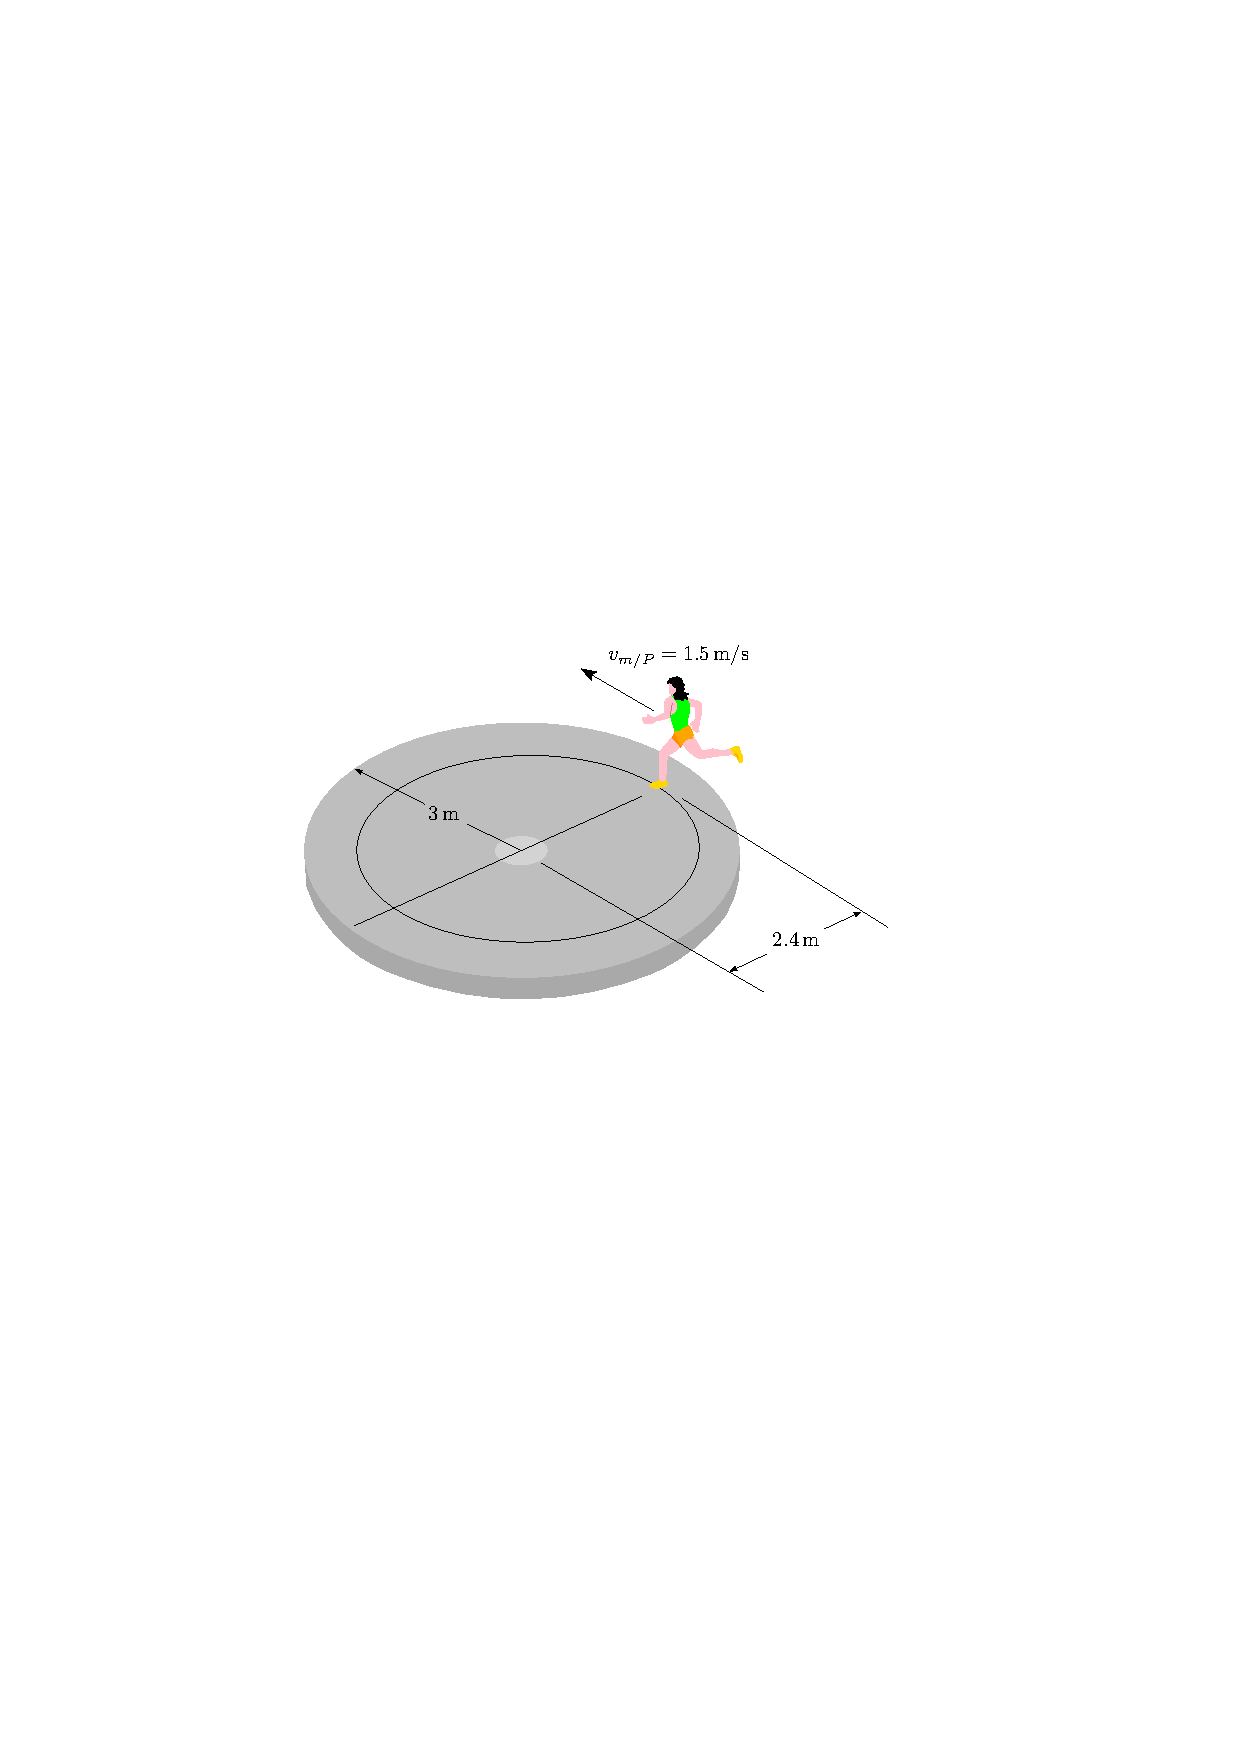
\includegraphics[scale=1.25]{../../images/draw_7_new}
\end{flushright}
